% !TeX engine = xelatex
\documentclass{ctexbeamer}
\usepackage{ctex}
\usepackage{booktabs}
\usepackage{svg}
\usepackage[style=authortitle-comp,backend=bibtex]{biblatex}
\usecolortheme{seagull}
\title{Deep-learning Based Models for Recommender Systems}
\subtitle{Wide \& Deep Learning for Regression/Classification Problems}
\author{Xinyi Li}
\date{\today}
\addbibresource{ref.bib}

\setbeamertemplate{sidebar right}{}
\setbeamertemplate{footline}{%
	\hfill\usebeamertemplate***{navigation symbols}
	\hspace{1cm}\insertframenumber{}/\inserttotalframenumber}
\begin{document}
\begin{frame}
	\titlepage
\end{frame}

\begin{frame}{Overview}
	\tableofcontents
\end{frame}

\section{History}
\begin{frame}{演化图谱\footfullcite{history_graph}}
	\begin{center}
	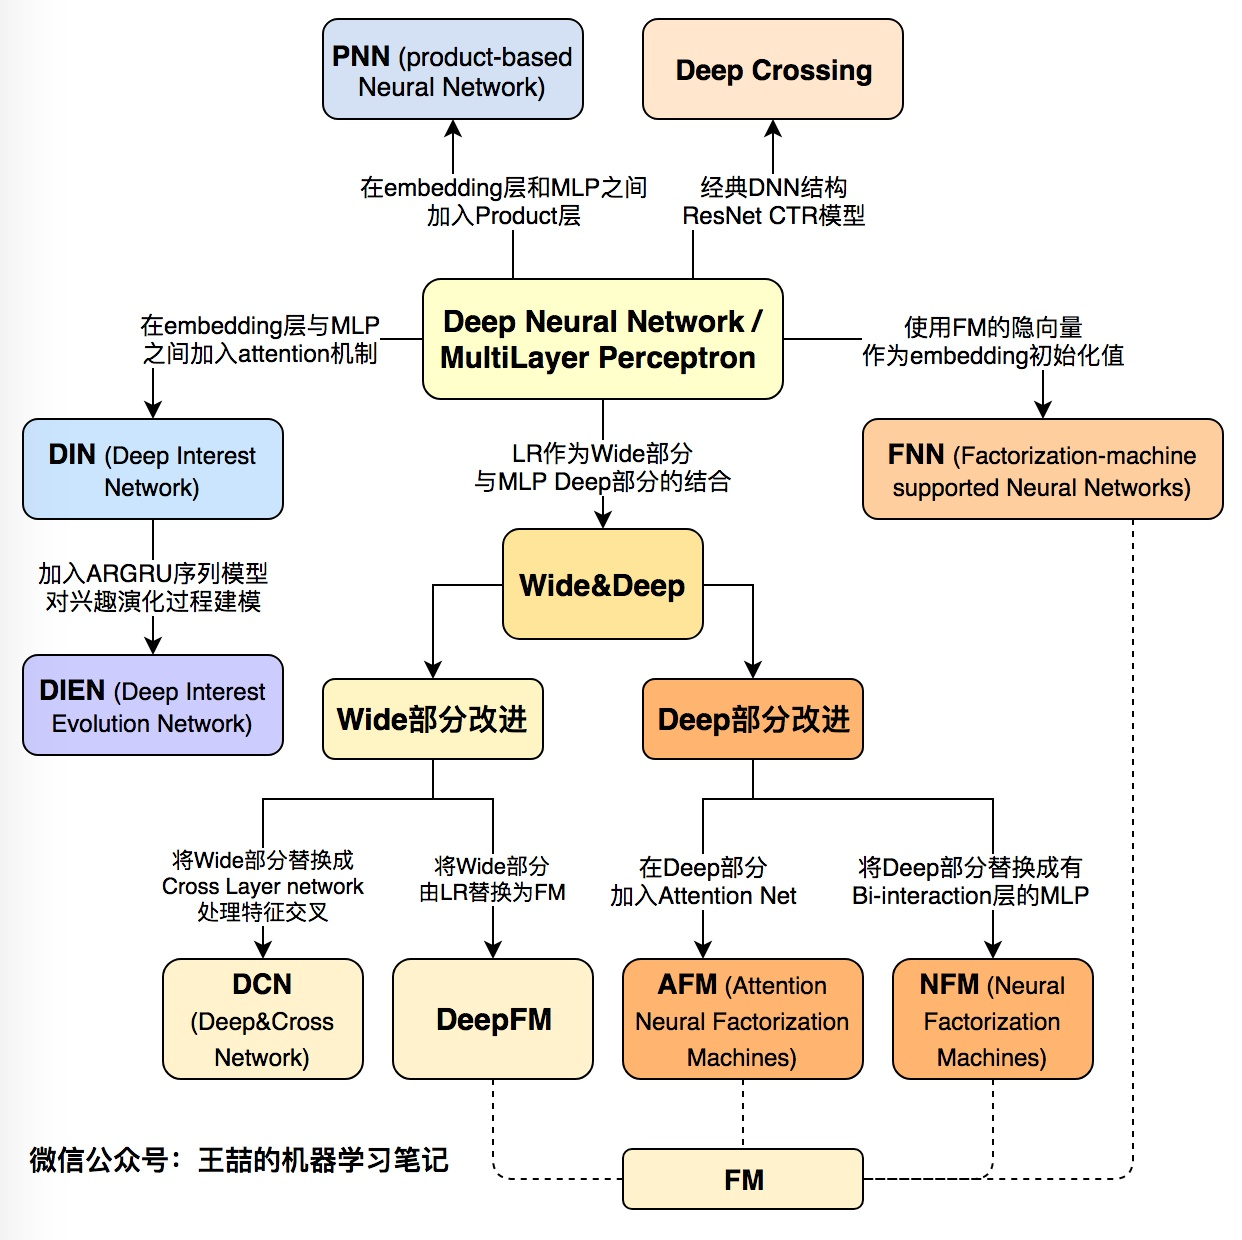
\includegraphics[width=.7\textwidth]{history}
\end{center}
\end{frame}

\subsection{Milestones}

\begin{frame}{Base Model: Deep Crossing \footfullcite{shan2016deep}}
	\framesubtitle{Microsoft}
	\begin{center}
		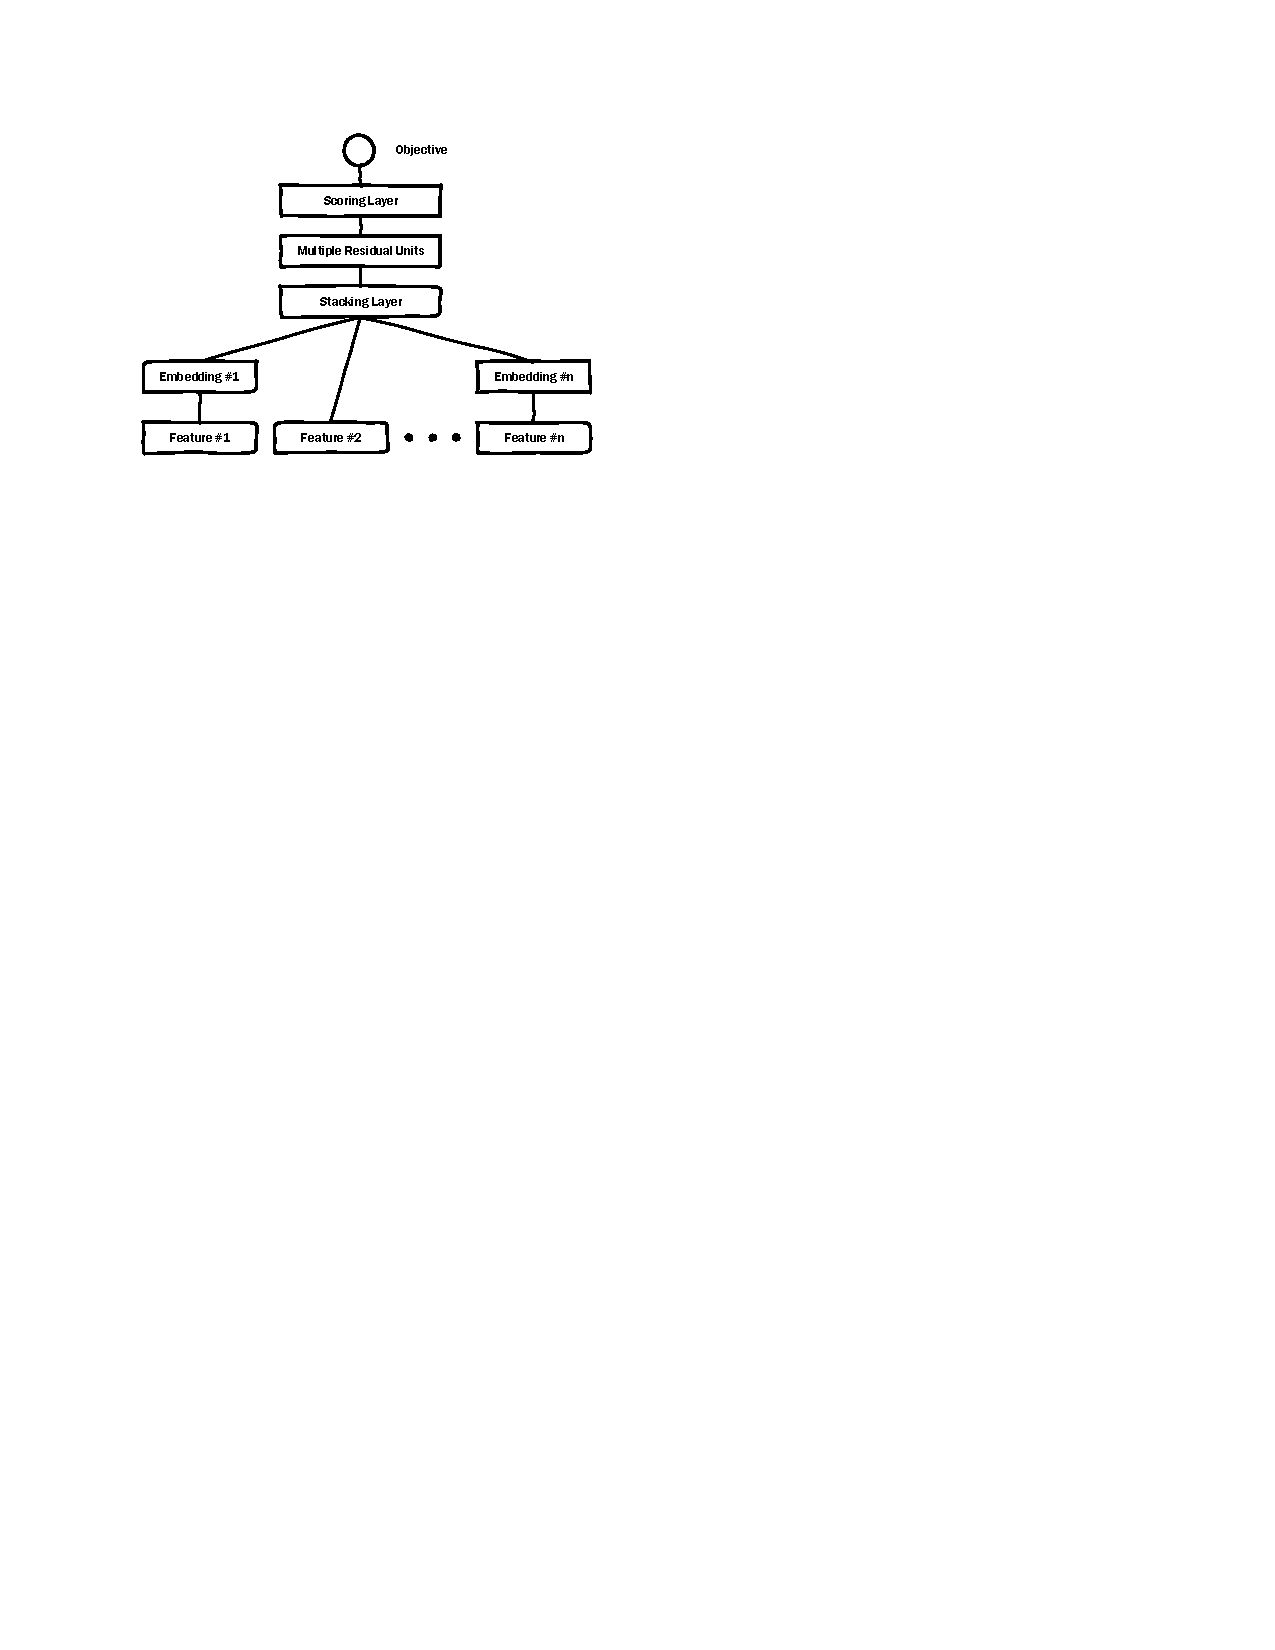
\includegraphics[width=.7\textwidth]{framework/deepcross}
	\end{center}
\end{frame}

\begin{frame}{Deep Crossing}
	\begin{block}{Scoring layer}
		\begin{itemize}
			\item objective: logloss
			\item sigmoid/softmax
		\end{itemize}
	\end{block}
	\begin{block}{Embedding layer}
		高维稀疏特征(id类,one-hot encode) {\color{red}{$\to$}} 低维稠密特征
		$$\mathbf{W}_j: (m_j \times n_j),\quad m_j {\color{red}{<}} n_j$$
		ReLu $$X_j^o = \max (\mathbf{0},\mathbf{W}_j X_j^I + \mathbf{b}_j )$$
	\end{block}
\end{frame}

\begin{frame}{Deep Crossing}
	\begin{block}{Stacking layer}
		concatenate: $X^O = [X_0^O,X_1^O,\cdots,X_K^O]$
	\end{block}
	\begin{block}{{\color{blue}{Residual}} layer}
		2 layers {\color{blue}{ReLu}} transform
		$$X^O = {\color{blue}{\cal F}}(X^I,\{\mathbf{W}_0,\mathbf{W}_1\},\{\mathbf{b}_0,\mathbf{b}_1\})+X^I$$
    \begin{center}
		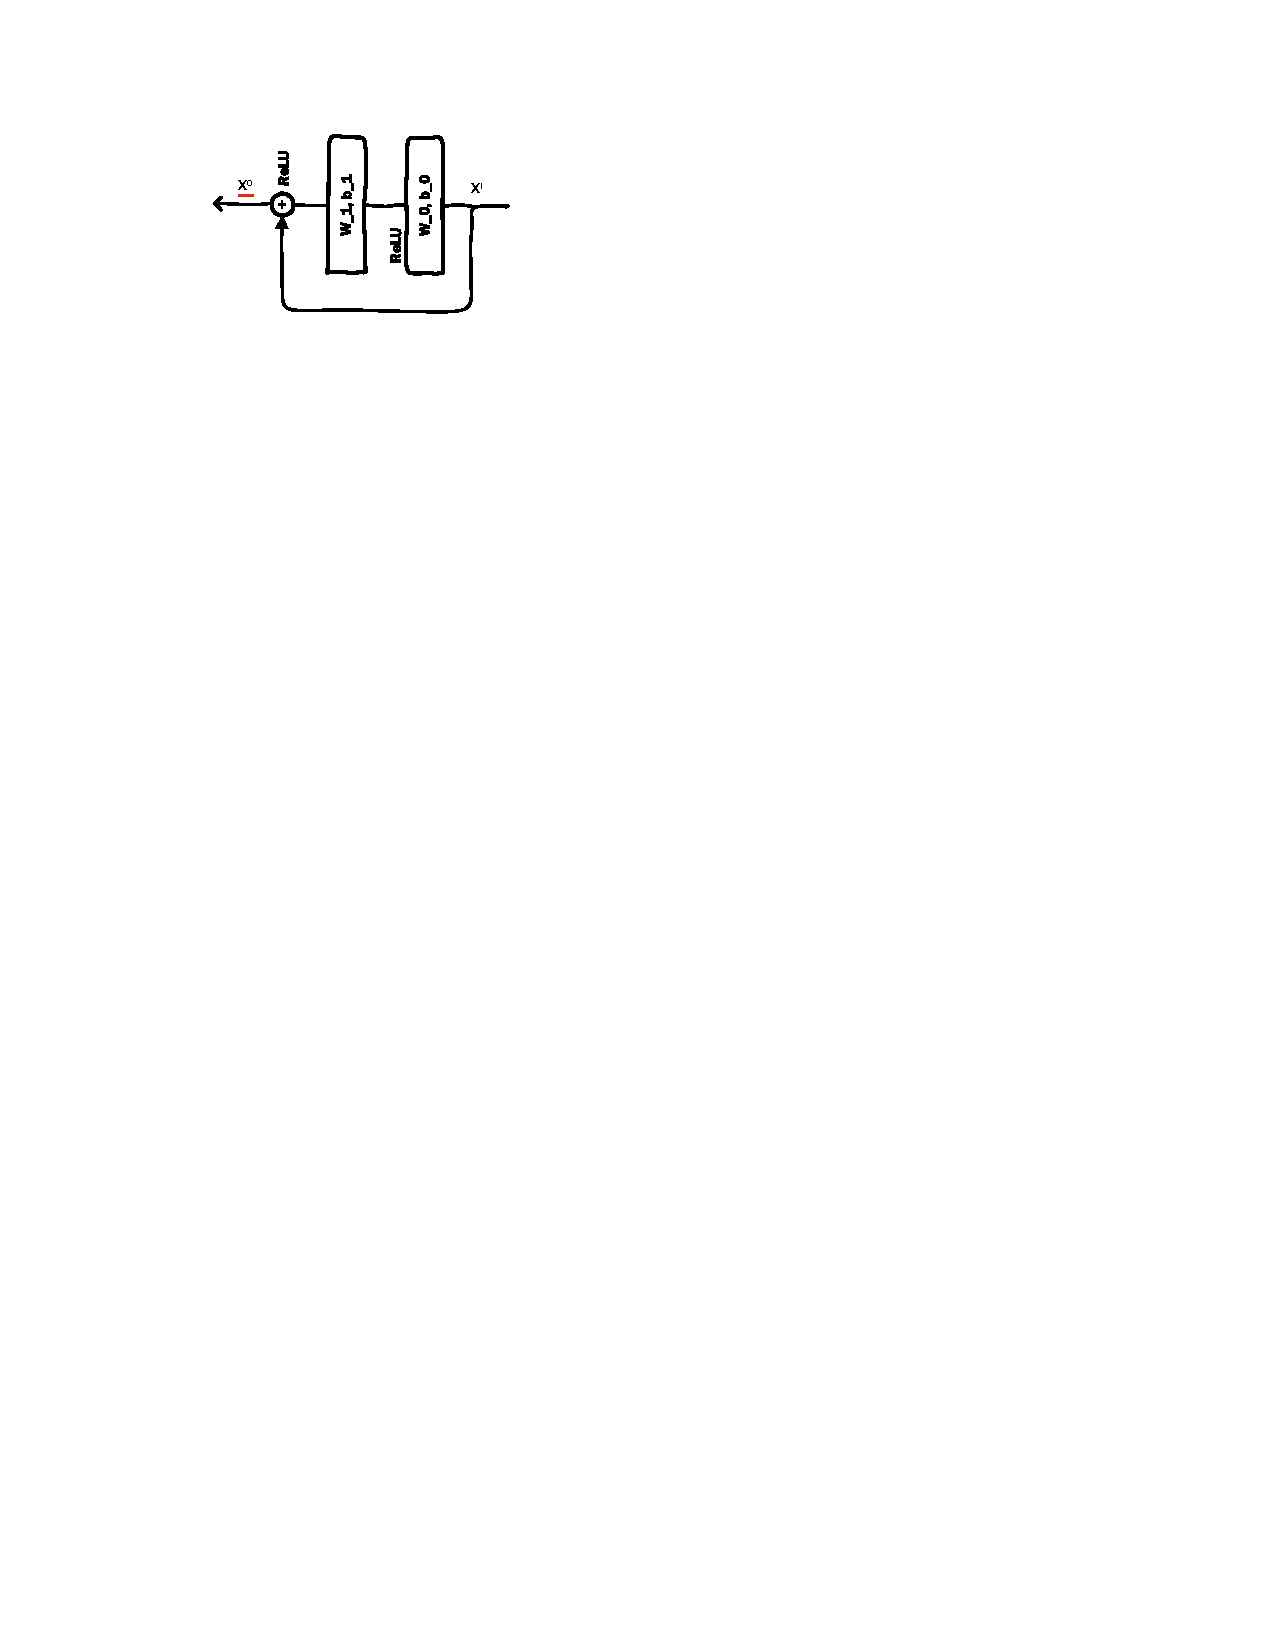
\includegraphics[width=.6\textwidth]{res_unit}
	\end{center}
	\end{block}
\end{frame}

\section{Wide \& Deep}
\subsection{Practice}

\section{Tools/Library}

\end{document}
